\documentclass[english]{article}

\usepackage{babel}
\usepackage{graphicx}
\usepackage{times}
\usepackage{pifont}
\usepackage[margin=1in]{geometry}
\usepackage{eurosym}
\usepackage{fancyhdr}
\usepackage[hidelinks]{hyperref}
\usepackage{float}
\usepackage{systeme,mathtools}

\pagestyle{fancy}
\fancyhf{}


%HEADER
%**************************************************************************************
\pagestyle{fancy}
\fancyhf{}
%**************************************************************************************
\lhead{Implementation of a strain gauge -based balance}		 	 
\rhead{Microsensors and Mechanics } 
\lfoot{EFA12SF}
\cfoot{\thepage}
\rfoot{Alexey Tukalo}
%**************************************************************************************

\date{}
\setlength\parindent{0pt}

\begin{document}

\title{\vspace{2in}Implementation of a strain gauge - based balance\\
\small for Microsensors and Mechanics \\
\vspace{0.5in}
\includegraphics{savonia.jpg}}

\nopagebreak
\maketitle


\vspace{3in}

\author{
\begin{flushright}
Alexey Tukalo,\\
EFA12SF,\\
Information Technology,\\
Savonia University of Applied Sciences
\end{flushright}
}

\date{\today}
\thispagestyle{empty}

\newpage
\setcounter{page}{1}
\setcounter{tocdepth}{2}
\tableofcontents

\newpage

%MAIN CONTENT ******************************************************************************************************************
\section{Introduction}
The report presents results of my laboratory work about calibration of a strain gauge - based balance sensor and measurements of weight with the sensor and LabVIEW software. The aim of the lab work is to learn how to connect digital multimeter to the computer and read the information on LabVIEW, the work also have to give me an experience with a strain gauge - based balance sensor, knowledge about connection of the circuit for this type of sensors.

\subsection{Implementation of a strain gauge -based balance}
A deformation of a body due to an amount of applied force can be described via strain. Strain Gauge Measurement – A Tutorial from National Instruments gives more scientific definition of strain: "strain ($\varepsilon$) is defined as the fractional change in length, as shown in Figure 1 below". The quantity can be positive and negative. A negative strain points to the compression of the object.\cite{str}

\begin{figure}[H]
\centerline{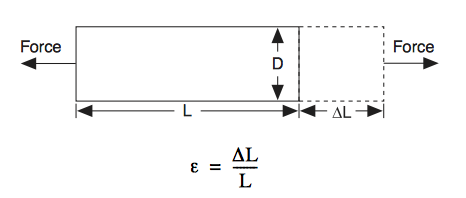
\includegraphics[scale=0.5]{labview/strait.png}}
\caption{Definition of Strain\cite{str}}
\end{figure}

A strain gauge - based balance is the most common technique for measuring of a strait. Usually, the sensor is made from materials which are able to change electrical resistance due to an amount of the materials strait. This type of sensors can be based on resistive and piezoresistive technologies.

\subsection{LabVIEW}

National Instruments developed software package for a visual programming called LabVIEW. The software was originally published for the Apple Macintosh in 1986. Today, the application is commonly used for a data acquisition, an instrument control and an industrial automation. The latest version of LabVIEW was released in 2015 for a variety of platforms\footnote{Microsoft Windows, Linux, and OS X}.\\

The programing language used in LabVIEW called G. It is a dataflow programing language. LabVIEW allows to build networks of nodes with different functionality connected via wires. The node is executed when the data flow reach it, so several nodes can be executed at the same time. The solution gives people without programing knowledge an opportunity to quickly implement their ideas by themselves.\cite{wiki}


\section{Materials}
During the laboratory work we used:

\begin{itemize}
\item strain gauge - based balance by Clas Ohlson
\item voltage amplifier by Stanford Research Systems
\item MyDAQ digital multimeter by National Instruments
\item power source
\item Alligator/Bullet connector x 2
\item BNC/Bullet connector x 2
\item Unknown mass
\item Known mass 1 (243 g) 
\item Known mass 2 (343 g)
\item Computer with LabView
\end{itemize}

All the equipments were provided to us by Savonia UAS.\cite{sv}

\section{Methods}

\subsection{Preparetion}
I started the lab from building of the circuit for the measurements in according with the circuit diagram shown on the picture 2.

\begin{figure}[H]
\centerline{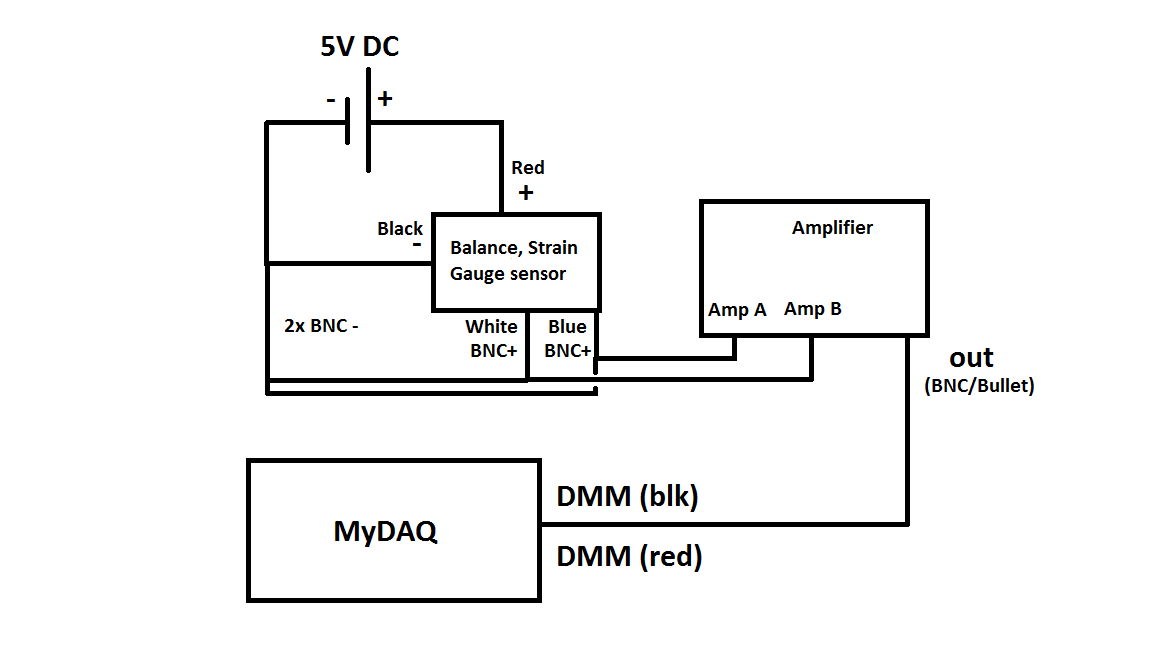
\includegraphics[scale=0.5]{labview/circuit}}
\caption{The curcuit diagram of the laboratory setup\cite{sv}}
\end{figure}

After that I adjusted the power supply and amplifier in according to the instruction of the experiment.\\

The last step of preparation is configuration of LabVIEW and MyDAQ digital multimeter to show the measured voltage in GUI of LabVIEW.

\subsection{Calibration}

The transfer function of our strain gauge - based balance is linear function(look at pic 3), so it is possible to define it with measurements of two known masses.

\begin{figure}[H]
\centerline{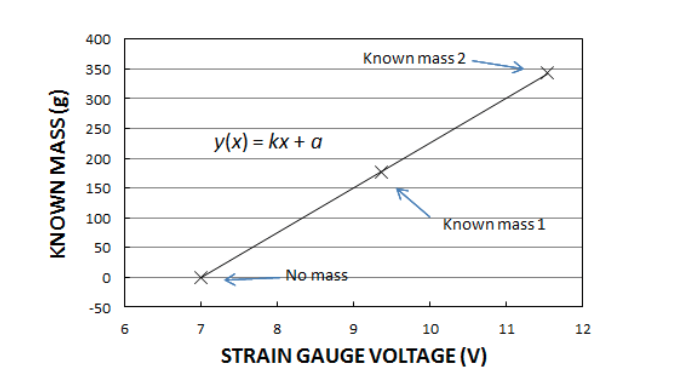
\includegraphics[scale=0.5]{labview/graph}}
\caption{Transfer function of the sensor\cite{sv}}
\end{figure}

\subsection{Measurements}
I made measurements for two different known masses, the results are shown on the table 1.

\begin{table}[H]
  \caption{Results of voltage measurments}
    \begin{center}
      \begin{tabular}{ c c }

        Mass & Output Voltage \\
        \hline\\
        0g & 5,005476V \\
        243g & 7,121662V \\
        343g & 7,98634V \\
      \end{tabular}
    \end{center}
  \end{table}
  
\subsection{Calculation}
  
Linear function is represented as $y(x) = kx + a$, so it is possible to use a system of linear equations for a two couple of x and y values to define the transfer function of the sensor. The derivation of the formulas for the values are shown below.\\

We can define one of unknown variables via another than and get normal linear equation. (Formula \ref{eq:system})

\begin{equation} \label{eq:system}
\systeme{y_1 = kx_1 + a, y_2 = kx_2 + a} \rightarrow \systeme*{y_1 - kx_1 = a, y_2 - kx_2 = a} \rightarrow y_1 - kx_1 = y_2 - kx_2 
\end{equation}

It is possible to easily solve the equation.(Formula \ref{eq:k})

\begin{equation} 
y_1 - y_2 = kx_1 - kx_2
\end{equation}
\begin{equation} 
y_1 - y_2 = k(x_1 - x_2)
\end{equation}
\begin{equation} \label{eq:k}
k = \frac{y_1 - y_2}{x_1 + x_2}
\end{equation}

The solution can be returned to the system and substituted to any of two original equation to calculate the second variable.(Formula \ref{eq:a})

\begin{equation} \label{eq:a}
\systeme*{k = \frac{y_1 - y_2}{x_1 + x_2}, a = y_1 - kx_1} \rightarrow \systeme*{k = \frac{y_1 - y_2}{x_1 + x_2}, a = y_1 - x_1\frac{y_1 - y_2}{x_1 - x_2}}
\end{equation}
Final formula is shown on equation \ref{eq:result}.

\begin{equation} \label{eq:result}
\systeme*{k = \frac{y_1 - y_2}{x_1 - x_2}, a = y_1 - x_1\frac{y_1 - y_2}{x_1 - x_2}}
\end{equation}

\subsection{Implementation}

It is possible to substitute the data from table 1 to the formula \ref{eq:result}. Let $x_1$ be 5,005476V and $y_1$ 0g when:

\begin{itemize}
\item $x_2$ be 7,121662V and $y_2$ 243g
\begin{equation} 
y = 114.8292 x - 574.7748
\end{equation}\label{eq:one}
\item $x_2$ be 7,98634V and $y_2$ 343g
\begin{equation} 
y = 115.0673 x - 575.9666
\end{equation}\label{eq:two}
\end{itemize}

I decided to use mean values of the results to reduce probability of errors.

\begin{equation} 
y = 114.9483 x - 575.371
\end{equation}\label{eq:final}

I used equation \ref{eq:final} to build the LabVIEWs flow for the data conversion, figure \ref{fig:lv}.

\begin{figure}[H]
\centerline{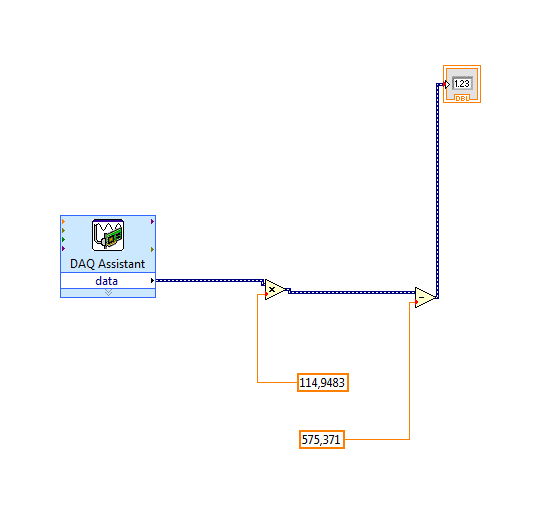
\includegraphics[scale=0.75]{labview/lv}}
\caption{Data flow for handling and converstion of the input\label{fig:lv}}
\end{figure}

\section{Results}

The LabVIEW interface for the sensor was tested by an unknown mass. In according with the lab work's instructions I had to measure the weight of my phone, but I did not have the phone with me at that moment, so I decided to measure the weight of my watch.\\

In according with the website of Casio, G-Shock DW5600E-1V's weight is 54g. In my measurment the result was 53.46g and in my point of view it is very accurate, because the watches has several scratches which can have a negative influence to the weight.\\

I also used my setup to measure known masses again, result are shown in table 2.

\begin{table}[H]
  \caption{Results of weigth measurments}
    \begin{center}
      \begin{tabular}{ c c c c }

        Original Mass & Calculeted Mass & Output Voltage & Error in persent \\
        \hline\\
        0g & -4,31092e-05g & 5,005476V & -\\
        243g & 243.2519g & 7,121662V & 0.1\%\\
        343g & 342.6452g & 7,98634V & 0.1\%\\
        54g & 53.46g & - & 1\%\\
      \end{tabular}
    \end{center}
  \end{table}


\section{Discussion}

During the lab work I learned how to connect digital multimeter to the computer and read the information on LabVIEW, I also got an experience with a strain gauge - based balance sensor, learned how to make connection of the circuit for this type of sensors. In addition I improved my skills in calibration of sensors. The most difficult part of the work for me was to make connection between myDAQ and the LabVIEW, because I am not very familiar with the software package and I have had some problems and errors at the step, but there were successfully solved via watching of tutorials at YouTube.\\

I think that the lab work was successful, I made setup in the right way, I connected the setup to a computer and successfully transferred the data into grams. I tested the sensor and my application with an unknown mass and I got quite accurate result.\\

Both measurements for known masses have errors about 0.1\% of the value, the measurement for my watch has a little bit higher error, about 1\%, but it can be result of the fact that the information on Casio's website is not enought  precise and my watches has several big scratches which reduce the mass.

\begin{thebibliography}{1}

   \bibitem{str} "Strain Gauge Measurement – A Tutorial" National Instruments
   
   \bibitem{sv} "Implementation of a strain gauge - based balance" Savonia UAS Lab Work instractions
   
   \bibitem{wiki} Wikipedia article about LabVIEW (16.12.2015)
  
  

\end{thebibliography}


\end{document}
